\section{Superposition}
\subsection{Principle of Superposition}
\begin{defn}{Principle of superposition}{}
When two or more waves of the \emph{same type} meet at a point at the same time, the displacement of the resultant wave is the \underline{vector sum} of the displacements of the individual waves at that point at that time.
\end{defn}

\subsection{Stationary Waves}
\begin{defn}{Node}{}
Region of destructive superposition where the two waves meet antiphase.

Displacement is permanently zero (or minimum amplitude).
\end{defn}

\begin{defn}{Antinode}{}
Region of constructive superposition where the two waves meet in phase. 

Displacement is maximum amplitude.
\end{defn}

Distance between two adjacent nodes / antinodes:
\[ d=\frac{1}{2}\lambda \]

\begin{defn}{Stationary wave}{}
A stationary wave is formed when two progressive waves of the \emph{same type} of \emph{equal amplitude}, \emph{equal frequency}, \emph{equal speed} travelling in opposite directions meet and undergo superposition with each other.
\end{defn}

\begin{itemize}
\item Wave profile does not advance.
\item Positions of wave elements oscillating with maximum amplitudes (antinodes) and minimum amplitudes (nodes) are fixed with time. 
\item Vibrational energy of the wave is not transmitted from one point to another.
\end{itemize}

Progressive vs stationary waves
\begin{table}[H]
\centering
\begin{tabular}{|p{2cm}|p{6.5cm}|p{6.5cm}|}
\hline
& \textbf{Progressive wave} & \textbf{Stationary wave} \\
\hline
Amplitude & Same amplitude for all particles in wave motion & Amplitude of oscillating particles varies from zero (at node) to a maximum (at antinode) \\
\hline
Frequency & Particles vibrate in SHM with frequency of progressive wave & Particles vibrate in SHM with frequency of stationary wave \\
\hline
Wavelength & Shortest distance between two points in phase & Twice the distance between a pair of adjacent nodes / antinodes \\
\hline
Phase & All particles within one wavelength have different phases & All particles within a loop vibrate in phase, paricles in adjacent loops are antiphase \\
\hline
Wave profile & Wave profile advances with the speed of wave & Wave profile does not advance \\
\hline
Energy & Energy is transported in the direction of travel of wave & Energy is stored within vibratory motion of stationary wave \\
\hline
\end{tabular}
\end{table}

Drawing of stationary waves: (draw the two extremes)


\subsubsection{Transverse stationary waves}
\paragraph{Stretched string}

\textbf{Experiment set-up:} String of length $L$ is stretched tightly between fixed supports. When plucked, progressive wave produces, reflected at fixed ends, travel backwards. Incident and reflected waves superpose to form a stationary wave.

\textbf{Node}: fixed ends

\begin{table}[H]
  \centering
  \begin{tabular}{|c|c|c|c|c|}
    \hline
    \textbf{Mode of vibration} & \textbf{Wavelength} & \textbf{Frequency} & \textbf{Harmonic} & \textbf{Overtone}\\
    \hline
    \begin{minipage}{.3\textwidth}
      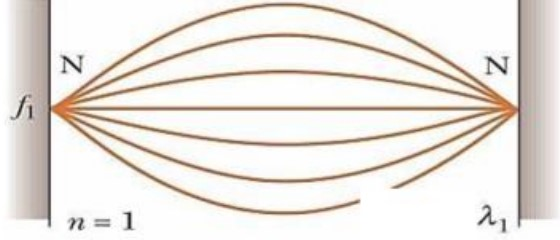
\includegraphics[width=\linewidth, height=30mm]{images/stretched_string_1.jpg}
    \end{minipage}
    & $\lambda_1=2L$ & $f_1=\dfrac{v}{\lambda_1}=\dfrac{v}{2L}$ & 1st & - \\
    \hline
    \begin{minipage}{.3\textwidth}
      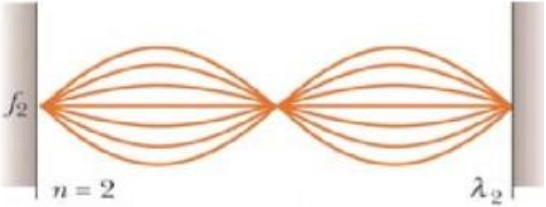
\includegraphics[width=\linewidth, height=30mm]{images/stretched_string_2.jpg}
    \end{minipage}
    & $\lambda_2=L$ & $f_2=\dfrac{v}{\lambda_2}=\dfrac{v}{L}=2f_1$ & 2nd & 1st \\
    \hline
    \begin{minipage}{.3\textwidth}
      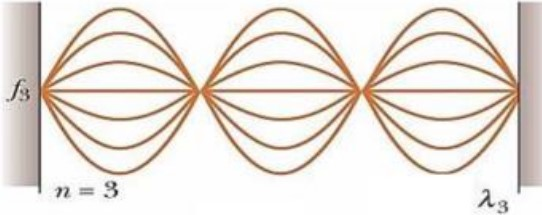
\includegraphics[width=\linewidth, height=30mm]{images/stretched_string_3.jpg}
    \end{minipage}
    & $\lambda_3=\dfrac{2}{3}L$ & $f_3=\dfrac{v}{\lambda_3}=\dfrac{3v}{2L}=3f_1$ & 3rd & 2nd \\
    \hline
  \end{tabular}
\end{table}

Integer number of lops must fit exactly into the length of the string, that is
\[ L=n\brac{\frac{\lambda}{2}} \]

Generalising, the $n$-th harmonic is given by 
\[ f_n = n\brac{\frac{v}{2L}} \]

\subsubsection{Longitudinal stationary waves}

\textbf{Experiment set-up:} Sound wave enters pipe via open end, travels from open end towards closed end, reflected when it hits wall of closed end.  Incident and reflected waves superpose to form a stationary wave.

\textbf{Node}: closed end\footnote{At the nodes, the air particles are not moving. Hence, they allow powder to collect at the nodes.}

\textbf{Antinode}: open end\footnote{At the antinodes, the air particles are moving with maximum amplitude. Hence, they ``push'' the powder away from the antinodes to the nodes.}

\paragraph{Closed pipe}

\paragraph{Open pipe}

\paragraph{End corrections} In practice, antinode at open end occurs \emph{slightly outside} the pipe.

\subsection{Diffraction}
\begin{defn}{Diffraction}{}
\underline{Spreading} of waves at edge of obstacle, or through slit, so that waves do not travel in straight lines.
\end{defn}

\begin{figure}[H]
    \centering
    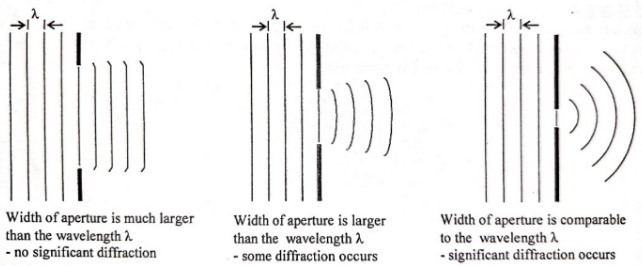
\includegraphics[width=15cm]{images/diffraction_waves.jpg}
\end{figure}

\textbf{Condition}: aperture size (size of slit) is comparable to wavelength (same order), i.e. $b\approx\lambda$.

\subsubsection{Single slit diffraction}
\paragraph{Mimima}
Positions of minima (points of zero intensity) occur at angles
\[ \sin\theta=m\frac{\lambda}{b} \]
where $m=\pm1,\pm2,\dots$

Hence position of first minima is at angle
\begin{equation}
\sin\theta=\frac{\lambda}{b}
\end{equation}

\paragraph{Rayleigh criterion}
Resolution of two objects is the ability to see as distinct two objects that are distinct.

\textbf{Rayleigh criterion} states that for two patterns to be \emph{just resolved}, the central maximum of one must lie on the first minimum of the other.

Minimum angle for two sources to be resolved:
\begin{equation}
\theta\approx\frac{\lambda}{b}
\end{equation}

\subsection{Interference}
\begin{defn}{Coherent waves}{}
Two waves have a \underline{constant phase difference} between them (with respect to time).
\end{defn}

\begin{defn}{Interference}{}
Superposition of \emph{coherent} waves which results in \underline{change in overall intensity}.
\end{defn}

\begin{defn}{Constructive interference}{}
When two waves meet \emph{in phase} at a point, resultant displacement is the \emph{sum} of magnitudes of individual displacements of the two waves.
\end{defn}

Path difference is a whole number of wavelengths, i.e. $n\lambda$.

\begin{defn}{Destructive interference}{}
When two waves meet \emph{antiphase} at a point, resultant displacement is the \emph{difference} of magnitude of individual displacements of the two waves.
\end{defn}

Path difference is an odd number of half wavelengths, i.e. $(n+\frac{1}{2})\lambda$

Conditions for two-source interference fringes to be \emph{observable}:
\begin{enumerate}
\item Waves must \emph{meet}
\item Waves must be \emph{coherent}
\item Waves have (approximately) equal amplitudes
\item Transverse waves must be either unpolarised or polarised in the same plane
\item Split separation is of same order as wavelength, i.e $b\approx\lambda$
\end{enumerate}


\subsubsection{Young's double slit diffraction}

% http://jcphysics.com/wp-content/uploads/2019/03/12-Superposition-Summary.pdf

\begin{equation}
\lambda=\frac{ax}{D}
\end{equation}

\subsection{Diffraction Grating}

\subsection*{Problems}
\begin{prbm}
A sound source of frequency $2500\:\unit{Hz}$ is placed several metres from a plane reflecting wall in a large chamber containing a gas. A microphone, connected to a c.r.o., is used to detect nodes and antinodes formed along the normal from the source to the wall. The microphone is moved from one node through $20$ antinodes to another node, across a distance of $1.90\:\unit{m}$.

Calculate the speed of sound in the gas.
\end{prbm}
\begin{solution}
The sequence of nodes and antinodes are given by
\[ N \quad A \quad N \quad \cdots \quad N \quad A \quad N \]
where the distance between two nodes is $d=\dfrac{\lambda}{2}$.

There are 20 half-wavelengths, so 
\[ 20\brac{\frac{\lambda}{2}}=1.90 \implies \lambda=0.190\:\unit{m} \]
The wavelength of the stationary wave is equal to that of the progressive wave that formed it.

Hence $v=f\lambda=(2500)(0.190)=\boxed{475\:\unit{m\,s^{-1}}}$.
\end{solution}

\pagebreak